\subsection{Planejamento de trajetória}

\subsubsection{Modelagem da superfície}\label{}
%Elael Modelo Polinomial multivarial -> extrapolado para a pá inteira
% PREMISSAS!!

Splines
Bézier Surface
Runge's phenomenon
Multivariate Polynomial fitting

\subsubsection{Cálculo dos paralelos}
% como subdividir em segmentos as regiões PREMISSAS!!
Na literatura, há diversas formas de dividir a superfície a ser revestida em
subregiões. Em \cite{from2010off}, por exemplo, um manipulador realiza a pintura
de uma superfície (\textit{spray gun}) cobrindo  subregiões de um plano, parametrização
da superfície (figura~\ref{fig::pal}). Como a superfície descrita na seção 

\begin{figure}[!ht]
	\centering	
	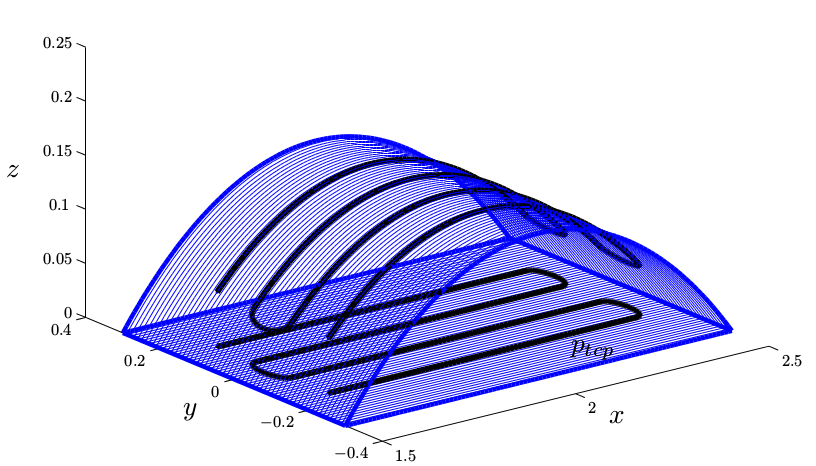
\includegraphics[width=.5\columnwidth]{figs/planejamento/pal.png}
	\caption{Subregiões de uma superfície.}
	\label{fig::pal}
\end{figure}

\subsubsection{Definição de caminho}
% Como transitar entre as paralelas de forma contínua